%\documentclass{beamer}
%\documentclass[c]{beamer}
 \documentclass[t]{beamer}
%\documentclass[b]{beamer}
\listfiles
\usepackage{tikz}
\usetikzlibrary{positioning}
\usetikzlibrary{decorations.text}
\usetikzlibrary{decorations.pathmorphing}
\usetikzlibrary{fit}
\usetikzlibrary{shapes}

\mode<presentation>
{
%  \usetheme[english]{KIT}
  \usetheme{Frankfurt}
  \usecolortheme{whale}
  \logo{
\includegraphics[height=1.cm]{logo-eps-converted-to.pdf}}
% \usetheme[usefoot]{KIT}
% \usetheme[deutsch]{KIT}

%%  \usefonttheme{structurebold}

  \setbeamercovered{transparent}

  %\setbeamertemplate{enumerate items}[circle]
  \setbeamertemplate{enumerate items}[ball]
}

\usepackage[english]{babel}
\date{15.09.14}
%\DateText

%\KITfoot{\parbox[t]{90mm}{\today:\qquad Dies ist eine sehr lange selbstdefinierte Fu\ss{}zeile -- Dies ist eine sehr lange selbstdefinierte Fu\ss{}zeile -- Dies ist eine sehr lange selbstdefinierte Fu\ss{}zeile}}


\usepackage[utf8]{inputenc}
\usepackage[T1]{fontenc}
\usepackage{array}
\usepackage{minted}

%\usenavigationsymbols
%\usenavigationsymbols[sfHhdb]
%\usenavigationsymbols[sfhHb]

\newminted{python}{gobble=4,linenos,fontsize=\scriptsize}
\newminted{bash}{gobble=4,fontsize=\scriptsize}

%\title[Python Interfaces for reactor codes]{Python Interfaces for Reactor Codes}
\title[HPMC final meeting]{PIRS: Python Interfaces for Reactor Simulations}
\subtitle{Current capabilities and selected results}

\author{A.Travleev}

\institute{Institute for Neutron Physics and Reactor Technology}


\begin{document}

\begin{frame}
  \maketitle
\end{frame}

\begin{frame}{Outline}
    \tableofcontents
\end{frame}


%%%%%%%%%%%%%%%%%%%%%%%%%%%%%%%%%%%%%%%%%%%%%%%%%%%%%%%%%%%%%%%%%%%%%%%%%%%%%%%%%%%%%%%%%%%%%%%%%%%%%
\section{What is PIRS and what it is for}
\begin{frame}\frametitle{What PIRS is}

    \begin{block}{PIRS: Python Interfaces for Reactor Simulations}

    A set of packages for \emph{Python} programming language, to facilitate
    \emph{interaction} with reactor calculation codes.
    \end{block}

    \begin{columns}
        \column{0.45\textwidth}
    \begin{block}{Python}
    \begin{itemize}

        \item www.python.org

        \item Free 

        \item Interpreted

        \item Big community

        \item Lot of packages 

    \end{itemize}
    \end{block}

        \column{0.45\textwidth}
    \begin{block}{Interaction with code}
    \begin{itemize}
        
        \item Model description

        \item Generation of Input file(s)

        \item Job submission

        \item Reading of calculation results

    \end{itemize}
    \end{block}
    \end{columns}
\end{frame}

\begin{frame}\frametitle{What PIRS is for}    

    
    \begin{itemize}

    \item Routine preparation of input files, reading output files 

    \item Framework for coupled calculations

    \end{itemize}

\end{frame}

\begin{frame}[fragile] \frametitle{PIRS concept}
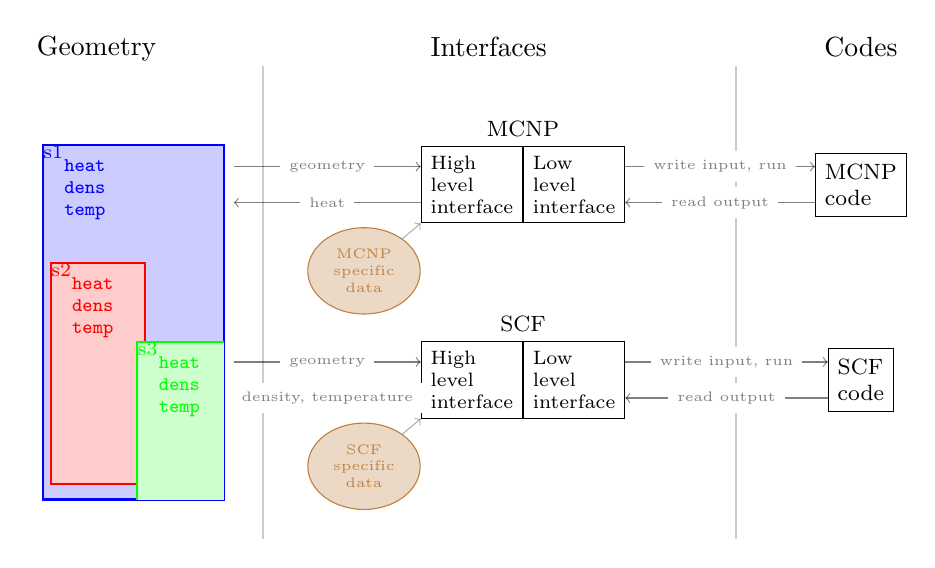
\begin{tikzpicture}
    %\draw[help lines, thin, color=blue!10] (0,0) grid (11,7);
    \tikzstyle{every node}=[font=\footnotesize]%, draw=black!10]%, draw=black, rounded corners, text centered]%, minimum height=1cm, text width=4cm]
    % Titles
    \tikzstyle{Titles}=[font=\normalsize, anchor=north west]
    \node[Titles] at (0,7) (t1) {Geometry};
    \node[Titles] at (5,7) (t2) {Interfaces};
    \node[Titles] at (10,7) (t3) {Codes};

    % vertical delimiters
    \tikzstyle{DelimiterLines}=[color=black!20, thick]
    \draw[DelimiterLines] (3, 6.5) -- +(0,-6cm);
    \draw[DelimiterLines] (9, 6.5) -- +(0,-6cm);

    % model example
    \coordinate (m1) at (0.2, 1);
    \coordinate (m2) at (2.5, 5.5);
    \coordinate (m3) at (0.3, 1.2);
    \coordinate (m4) at (1.5, 4.0);
    \coordinate (m5) at (1.4, -1);
    \coordinate (m6) at (2.7, 3.0);
    \node[opacity=0., fit=(m1) (m2)] (model) {};
    \begin{scope}% scope here while clipping.
        \path[clip] 
            [preaction = {draw=blue,thick, fill=blue!20}]
            (m1) rectangle (m2);
        \path[thick, fill=red!20,   draw=red]   (m3) rectangle (m4);
        \path[thick, fill=green!20, draw=green] (m5) rectangle (m6);
    \end{scope}
    
    \tikzstyle{SolidLabels}=[align=right,font=\scriptsize, opacity=0., text opacity=1., inner sep=0., anchor=north west]
    \tikzstyle{MeshLabels}=[SolidLabels,font=\scriptsize\tt]
    \node[SolidLabels, text=blue] at (m1 |- m2) (s1) {s1};
    \node[SolidLabels, text=red]   at (m3 |- m4) (s2) {s2};
    \node[SolidLabels, text=green] at (m5 |- m6) (s3) {s3};

    \node[MeshLabels,  text=blue,  below right=0mm of s1] (m1) {heat\\dens\\temp};
    \node[MeshLabels,  text=red,   below right=0mm of s2] (m2) {heat\\dens\\temp};
    \node[MeshLabels,  text=green, below right=0mm of s3] (m3) {heat\\dens\\temp};

    % % interfaces
    \tikzstyle{Interfaces}=[draw=black,rectangle split, rectangle split parts=2, rectangle split horizontal=true, minimum height=0.8cm, align=left,font=\scriptsize]
    \tikzstyle{SpecData}=[color=brown, draw, fill, ellipse, align=center, font=\tiny, opacity=1, fill opacity=0.3, text opacity=1.]

    \node[Interfaces, anchor=west, label=above:MCNP] at (5, 5) (mi) {High\\level\\interface \nodepart{second} Low\\level\\interface};
    \node[SpecData, below left=3mm of mi] (msd) {MCNP\\specific\\data};

    \node[Interfaces, below=15mm of mi, label=above:SCF] (si) {High\\level\\interface \nodepart{second} Low\\level\\interface};
    \node[SpecData, below left=3mm of si] (ssd) {SCF\\specific\\data};



    % codes
    \tikzstyle{Codes}=[draw=black, minimum height=0.8cm, align=left]
    \node[Codes, align=left] at (t3 |- mi) (mcnp) {MCNP\\code};
    \node[Codes, align=left] at (t3 |- si) (scf)  {SCF\\code};


    %% connections
    \tikzstyle{ConnectionNodes}=[font=\tiny, fill=white, fill opacity=1., text opacity=0.5, align=center]
    \tikzstyle{ConnectionLines}=[opacity=0.5]

    % model -- MCNP interface
    \draw[ConnectionLines, ->] (model.east |- mi.170) -- node[ConnectionNodes] {geometry} (mi.170);
    \draw[ConnectionLines, <-] (model.east |- mi.190) -- node[ConnectionNodes] {heat}     (mi.190);

    % MCNP interface -- MCNP
    \draw[ConnectionLines, ->] (mi.10)  -- node[ConnectionNodes] {write input, run} (mcnp.west |- mi.10);
    \draw[ConnectionLines, <-] (mi.-10) -- node[ConnectionNodes] {read output}      (mcnp.west |- mi.-10);

    % model -- SCF interface
    \draw[ConnectionLines, ->] (model.east |- si.170) -- node[ConnectionNodes] {geometry}             (si.170);
    \draw[ConnectionLines, <-] (model.east |- si.190) -- node[ConnectionNodes] {density, temperature} (si.190);

    % SCF interface -- SCF
    \draw[ConnectionLines, ->] (si.10)  -- node[ConnectionNodes] {write input, run} (scf.west |- si.10);
    \draw[ConnectionLines, <-] (si.-10) -- node[ConnectionNodes] {read output}      (scf.west |- si.-10);

    % code specific data
    \draw[ConnectionLines, ->, opacity=0.3] (msd) -- (mi.south west);
    \draw[ConnectionLines, ->, opacity=0.3] (ssd) -- (si.south west);



\end{tikzpicture}

\end{frame}




%%%%%%%%%%%%%%%%%%%%%%%%%%%%%%%%%%%%%%%%%%%%%%%%%%%%%%%%%%%%%%%%%%%%%%%%%%%%%%%%%%%%%%%%%%%%%%%%%%%%%
% \section{Introduction to Python}
% \begin{frame}[fragile]
    \frametitle{Python Interpreter}

    \begin{bashcode}
        $ python --version
        Python 2.7.3
        $ python
    \end{bashcode}
        
    \begin{pythoncode}
        >>> from math import pi
        >>> print pi
        3.14159265359
        
        >>> from pirs.solids import Box
        >>> b = Box()
        >>> b.X = 5

        >>> print b
        >>> print repr(b)

        >>> help(b)
        >>> dir()
        >>> dir(b)
    \end{pythoncode}

\end{frame}

\begin{frame}[fragile]
    \frametitle{Python script}

    \begin{bashcode}
        $ python script.py
    \end{bashcode}
        
    \begin{pythoncode}
        l = [1, 2, 3, 4, 5]
        s = 0
        for e in l:
            s += e
            print e, s

        for c in 'abs':
            print c

    \end{pythoncode}

\end{frame}


%%%%%%%%%%%%%%%%%%%%%%%%%%%%%%%%%%%%%%%%%%%%%%%%%%%%%%%%%%%%%%%%%%%%%%%%%%%%%%%%%%%%%%%%%%%%%%%%%%%%%
%\section{How to install PIRS}
%%%%%%%%%%%%%%%%%%%%%%%%%%%%%%%%%%%%%%%%%%%%%%%%%%%%%%%%%%%%%%%%%%%%%%%%%%%%%%%%%%%%%%%%%%%%%%%%%%%%%%
\subsection{Prerequisites}

\begin{frame}{Python version}

    \begin{block}{Python 2 or 3?}
    "Python 2.x is legacy, Python 3.x is the present and future of the language" from www.python.org/doc 
    \end{block}

    \begin{block}{PIRS uses Python 2.x}
    PIRS is developed for Python 2.6.x or above. Not for Python 3.x!
    \end{block}
                
    Usually Python 2.6.x or 2.7.x is already installed. If not, can be
    installed using OS installer (e.g. Ubuntu Software Center), or compiled
    from sources.

\end{frame}

\begin{frame}[fragile]
    \frametitle{Required packages}
    \begin{block}{uncertainties} 
        Needed to preserve information about errors in MC calculations. 

        \begin{bashcode*}{gobble=12}
            $ wget https://pypi.python.org/.../uncertainties-2.4.6.tar.gz
            $ tar -xzf uncertainties-2.4.6.tar.gz
            $ cd uncertainties-2.4.6
            $ python setup.py install --user
        \end{bashcode*}
    \end{block}

    \begin{block}{matplotlib}
        Optional. Needed to plot geometry and results of calculations. 
        
        Simplest way to install -- using OS installer. Compilation from sources
        is difficult due to lot of dependencies.
    \end{block}

\end{frame}

\begin{frame}[fragile]
    \frametitle{Environmental variables}
    Several enviromental variables should be defined.

    \begin{block}{\$DATAPATH}
        Path to xsdir file and files with cross-sections.

        \begin{bashcode}
            $ echo $DATAPATH
            /home/data/mcnp
        \end{bashcode}
    \end{block}

    \begin{block}{\$MCNP}
        Path to MCNP executable

        \begin{bashcode}
            $ echo $MCNP
            /home/bin/mcnp5_linux_i386_omp
        \end{bashcode}
    \end{block}

    \begin{block}{\$SCF}
        Path to SCF executable

        \begin{bashcode}
            $ echo $SCF
            /home/bin/scf25_intel
        \end{bashcode}
    \end{block}
\end{frame}

%%%%%%%%%%%%%%%%%%%%%%%%%%%%%%%%%%%%%%%%%%%%%%%%%%%%%%%%%%%%%%%%%%%%%%%%%%%%%%%%%%%%%%%%%%%%%%%%%%%%%
\subsection{PIRS installation}

\begin{frame}[fragile]
    \frametitle{How to install PIRS}
    
    \begin{block}{Standard method}
        \begin{bashcode}
            $ tar -xzf pirs-0.2a.0.tar.gz
            $ cd pirs-0.2a.0
            $ python setup.py install --user
        \end{bashcode}

        Dependencies should be installed separately.
    \end{block}


    \begin{block}{2-nd method}
        It uses pip -- python package installer that is not available by default.

        \begin{bashcode}
            $ pip install pirs-0.2a.0.tar.gz --user
        \end{bashcode}

        Dependencies will be installed by pip, if necessary.
    \end{block}

    \begin{block}{Test}
        \begin{pythoncode}
            from pirs.solids import Box
            from pirs import McnpInterface
            b = Box()
            m = McnpInterface(b)
            m.run('r')
        \end{pythoncode}
    \end{block}

\end{frame}





%%%%%%%%%%%%%%%%%%%%%%%%%%%%%%%%%%%%%%%%%%%%%%%%%%%%%%%%%%%%%%%%%%%%%%%%%%%%%%%%%%%%%%%%%%%%%%%%%%%%%
%\section{Package content of PIRS}
%\begin{frame}[fragile]
    \frametitle{PIRS classes and functions}

    \begin{block}{Classes for geometry description}
        \begin{pythoncode}
            from pirs.solids import zmesh
            from pirs.solids import Cylinder, Box, Sphere
        \end{pythoncode}
    \end{block}

    \begin{block}{High-level interfaces}
        \begin{pythoncode}
            from pirs import McnpInterface
            from pirs import ScfInterface
        \end{pythoncode}
    \end{block}

    \begin{block}{Low-level interface to MCNP}
        \begin{pythoncode}
            from pirs.mcnp import Material, MaterialCollection
            from pirs.mcnp import MeshTally, TallyCollection
            from pirs.mcnp import Xsdir
            from pirs.mcnp import Surface, Volume, SurfaceCollection
            from pirs.mcnp import Cell, Model
            from pirs.mcnp import xs_interpolation
        \end{pythoncode}
    \end{block}
\end{frame}

\begin{frame}[fragile]
    \frametitle{PIRS classes and functions}

    \begin{block}{Low-level interface to SCF}
        \begin{pythoncode}
            from pirs.scf2 import Input
            from pirs.scf2 import read_output, OutputTable
        \end{pythoncode}
    \end{block}

    \begin{block}{Tools}
        \begin{pythoncode}
            from pirs.tools import LoadMap
            from pirs.tools import load, dump

            from pirs.tools.plots import MeshPlotter, colormap
        \end{pythoncode}
    \end{block}

    \begin{block}{Base classes}
        Not needed to end-user of PIRS.
        \begin{pythoncode}
            from pirs.core.tramat import Nuclide, Mixture, zai
            from pirs.core.trageom import Vector3, pi, pi2
            from pirs.core.scheduler import Job, Scheduler, enva, WorkPlace, InputFile
        \end{pythoncode}
    \end{block}

\end{frame}



%%%%%%%%%%%%%%%%%%%%%%%%%%%%%%%%%%%%%%%%%%%%%%%%%%%%%%%%%%%%%%%%%%%%%%%%%%%%%%%%%%%%%%%%%%%%%%%%%%%%%
\section{PIRS current capabilities}
\begin{frame}[fragile]
    \frametitle{PIRS current capabilites}

    \begin{block}{Geometry definition}
    \begin{itemize}
        \item Geometry described by 
            \begin{itemize}
                \item boxes with facets perpendicular to coordinate axes
                \item cylinders with axes parallel to z (vertical) axis
            \end{itemize}
        \item Dependent variables vertical distribution are presented by piece-wise constant functions
            \begin{itemize}
                \item heat deposition
                \item temperature
                \item material density
            \end{itemize}
    \end{itemize}
    \end{block}

    \begin{block}{Low-level interfaces}
    Classes to represent code input data, to start code, read code output
    \begin{itemize}
        \item MCNP 5
        \item SCF 2.5
    \end{itemize}
    \end{block}
\end{frame}

\begin{frame}[fragile]
    \frametitle{PIRS current capabilites (contd.)}
    \begin{block}{High-level interfaces}
    Classes to convert geometry to code-specific representation, start calculations and 
    put results back to geometry.
    \begin{itemize}
        \item MCNP 5: any geometry can be converted into MCNP input file. 
        \item SCF 2.5: for square bundle of vertical rods only. 
    \end{itemize}
    \end{block}

    \begin{block}{Utils}
    \begin{itemize}
        \item geometry plotter
        \item plotter of vertical distributions
        \item dump and load models to and from hard drive    
    \end{itemize}
    \end{block}
\end{frame}



%%%%%%%%%%%%%%%%%%%%%%%%%%%%%%%%%%%%%%%%%%%%%%%%%%%%%%%%%%%%%%%%%%%%%%%%%%%%%%%%%%%%%%%%%%%%%%%%%%%%%
\section{Example}
\subsection{Geometry description}
\begin{frame}[fragile]
    \frametitle{Geometry I}
    \inputminted[frame=single,fontfamily=tt,fontsize=\footnotesize]{python}{examples/geom1.py}
\end{frame}

\begin{frame}\frametitle{Geometry I: plots}
    \begin{columns}
        \column{0.3\textwidth}
            {\tiny z plane}
            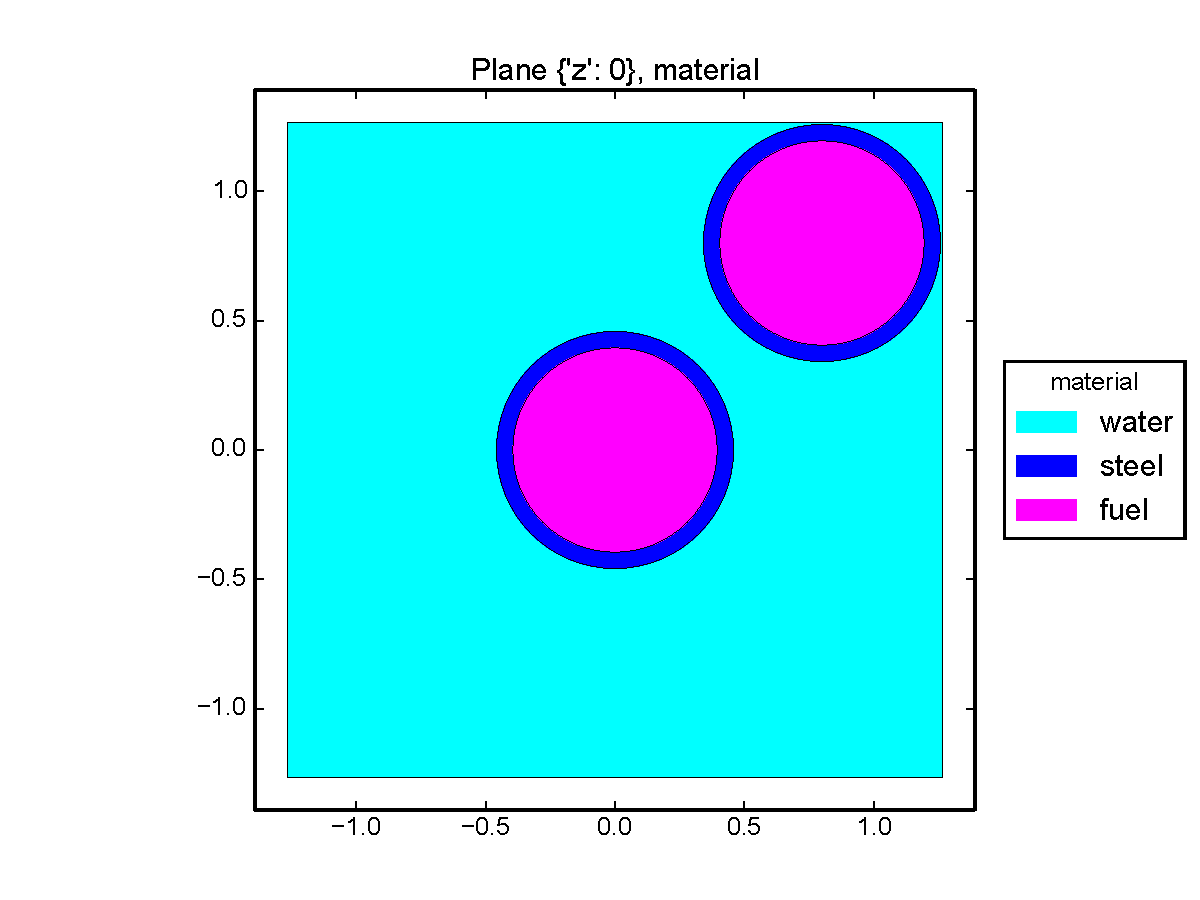
\includegraphics[width=\textwidth]{examples/geom1_pz.pdf}
        \column{0.3\textwidth}
            {\tiny x plane}
            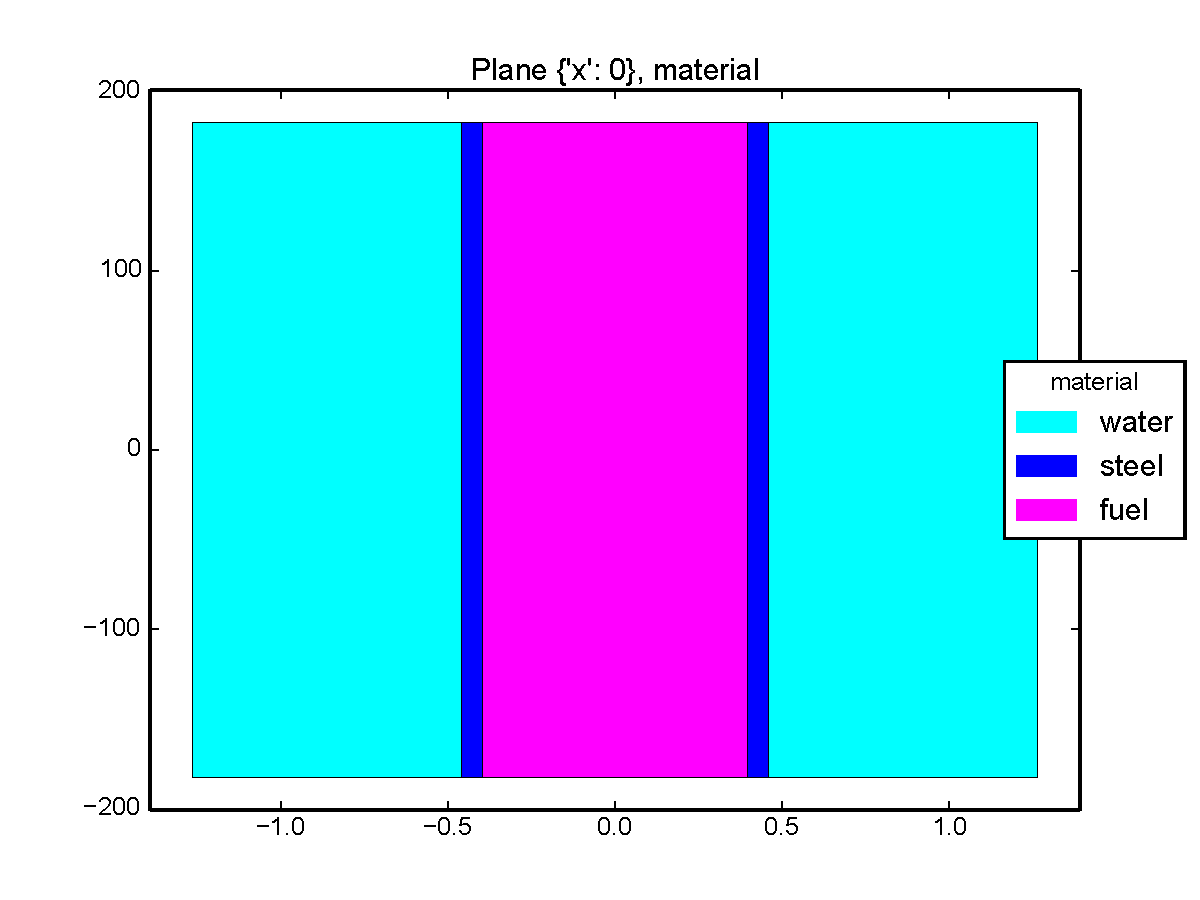
\includegraphics[width=\textwidth]{examples/geom1_px.pdf}
        \column{0.3\textwidth}
            {\tiny y plane}
            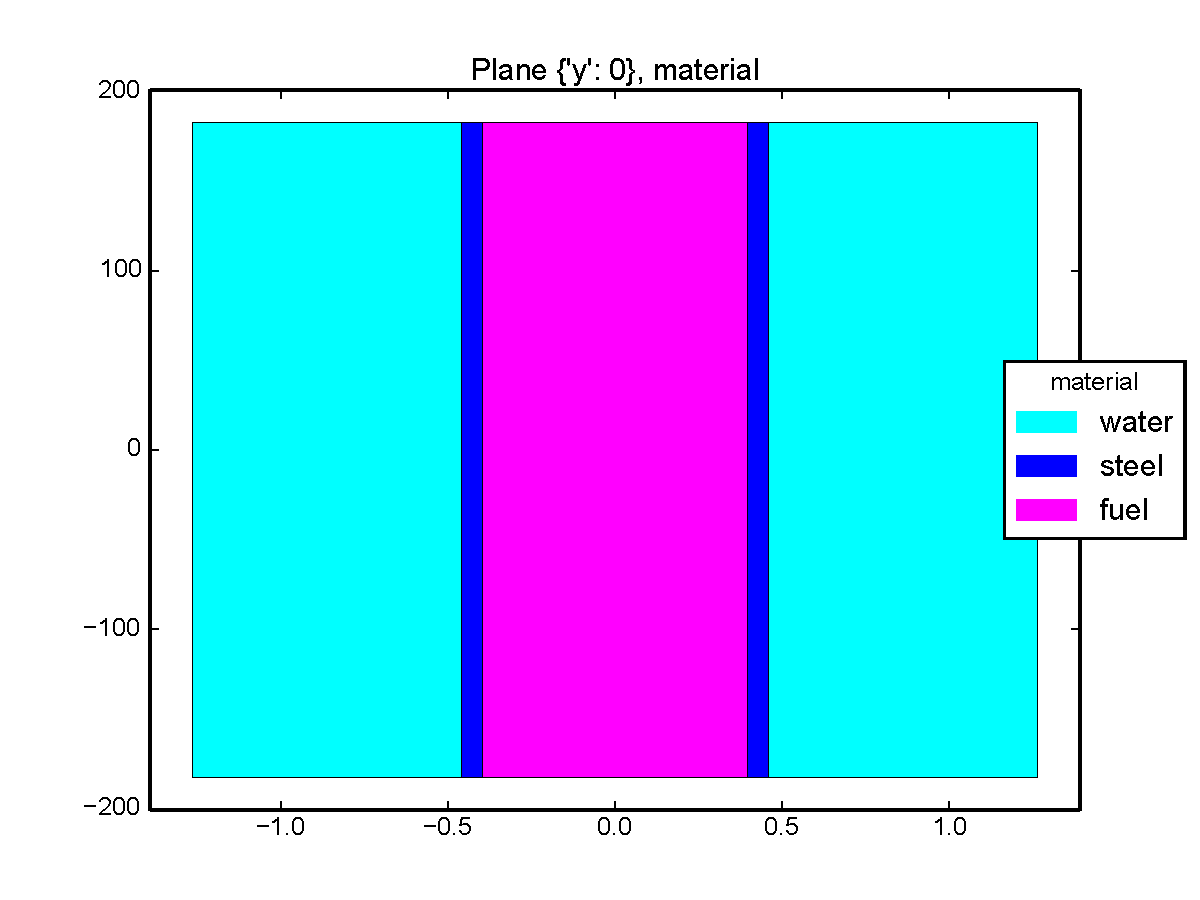
\includegraphics[width=\textwidth]{examples/geom1_py.pdf}
    \end{columns}
\end{frame}

\begin{frame}[fragile]
    \frametitle{System variables}
    \inputminted[frame=single,fontfamily=tt,fontsize=\scriptsize]{python}{examples/geom2.py}
\end{frame}

\begin{frame}\frametitle{System variables: plot}
    \begin{columns}
        \column{0.5\textwidth}
        {\tiny density at plane y=0}
        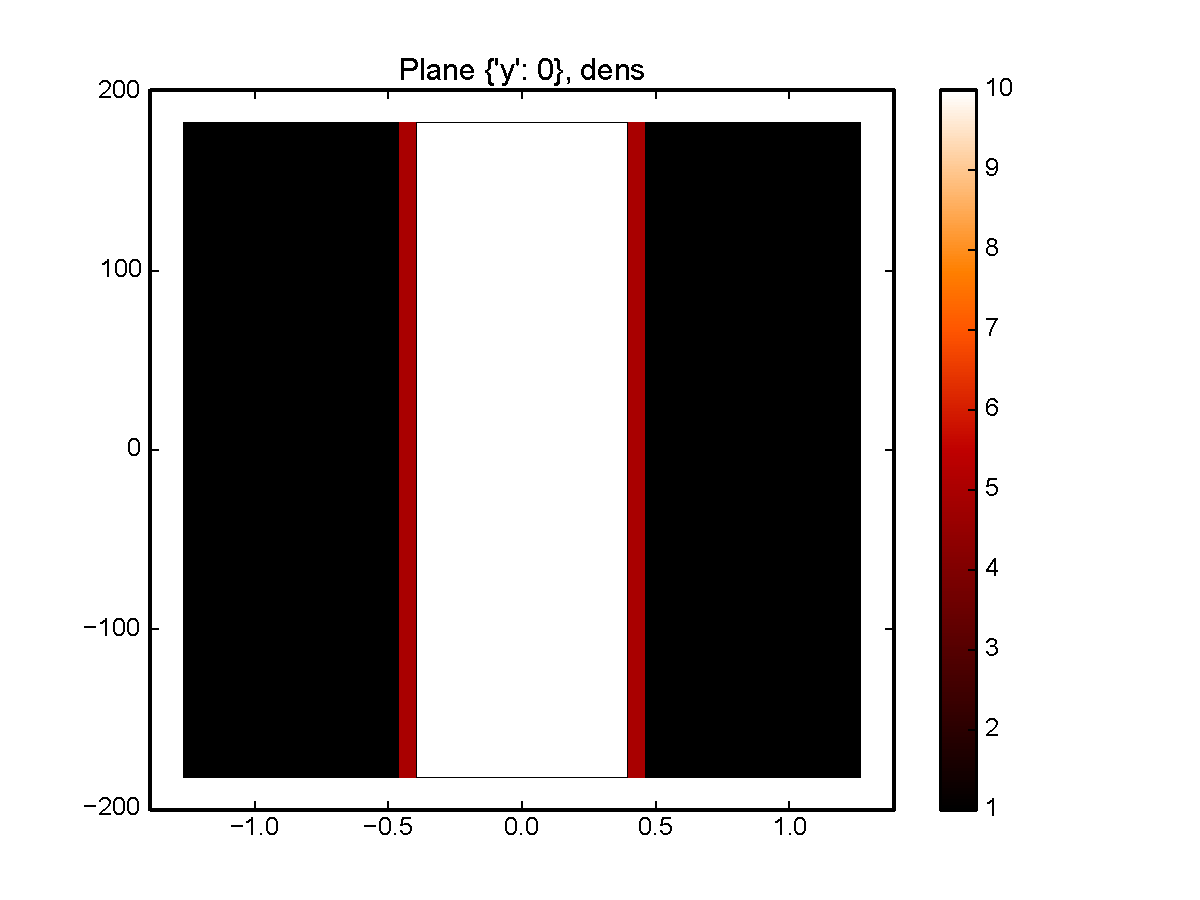
\includegraphics[width=\textwidth]{examples/geom2_d.pdf}
        \column{0.5\textwidth}
        {\tiny temperature at plate y=0}
        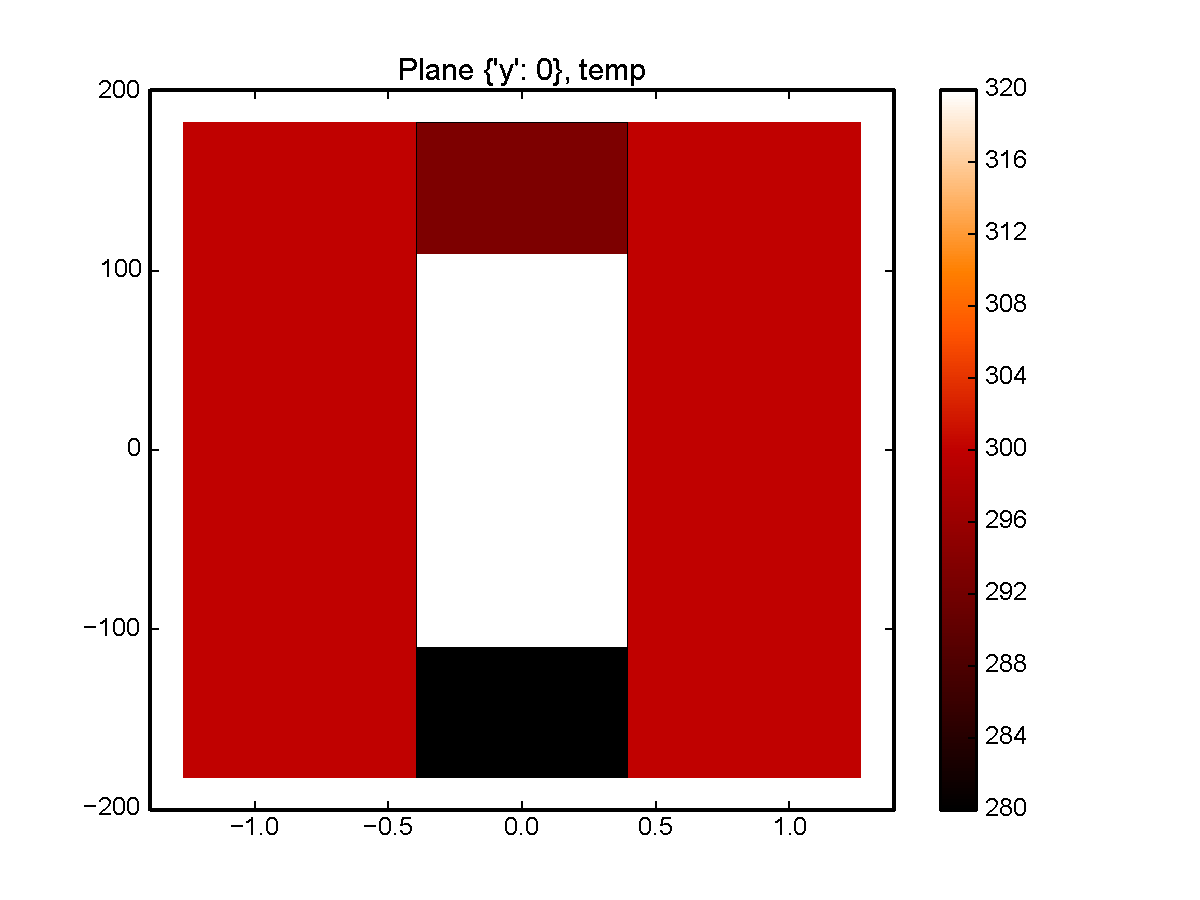
\includegraphics[width=\textwidth]{examples/geom2_t.pdf}
    \end{columns}
\end{frame}

\begin{frame}[fragile]
    \frametitle{Geometry II}
    \inputminted[frame=single,fontfamily=tt,fontsize=\footnotesize]{python}{examples/geom3.py}
\end{frame}

\begin{frame}\frametitle{Geometry II: plots}
    \begin{columns}
        \column{0.3\textwidth}
            {\tiny z plane}
            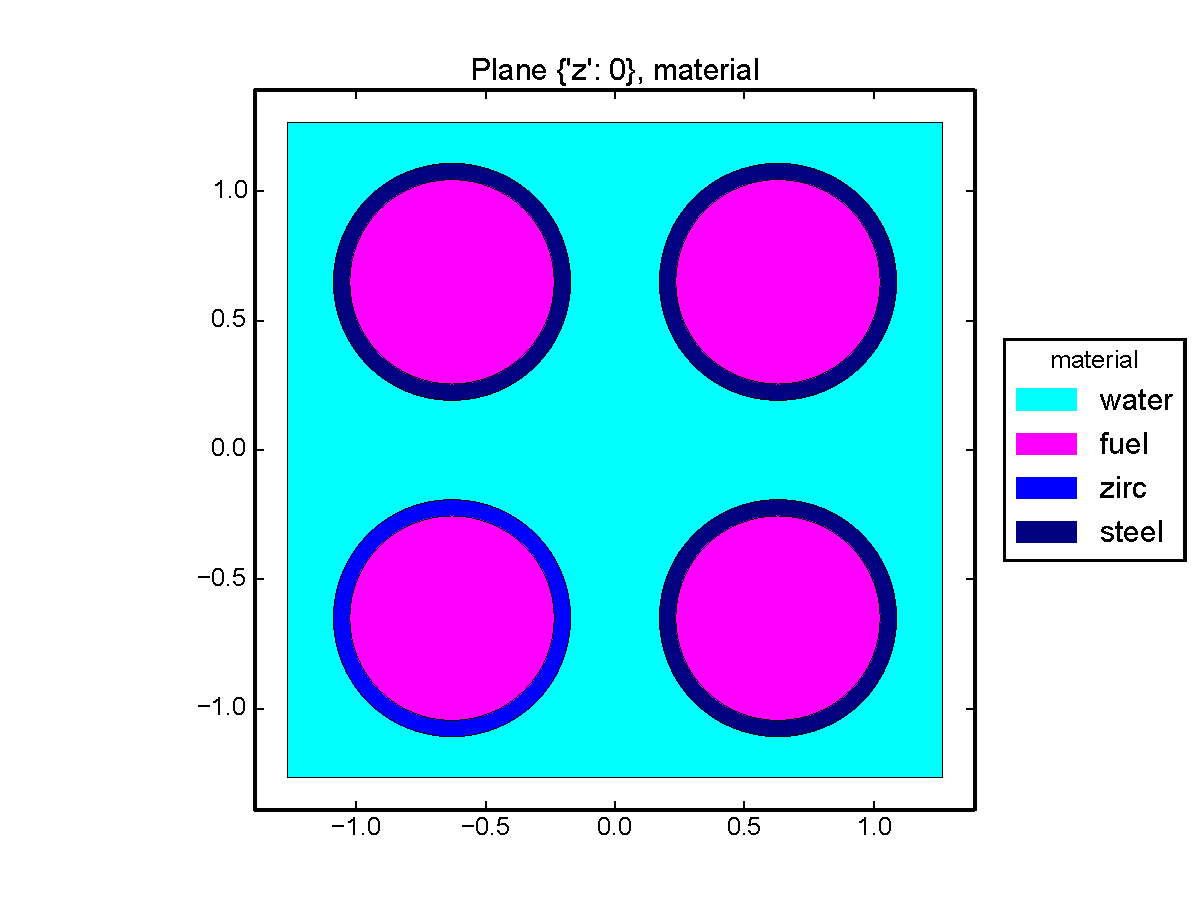
\includegraphics[width=\textwidth]{examples/geom3_pz.pdf}
        \column{0.3\textwidth}
            {\tiny x plane at -1}
            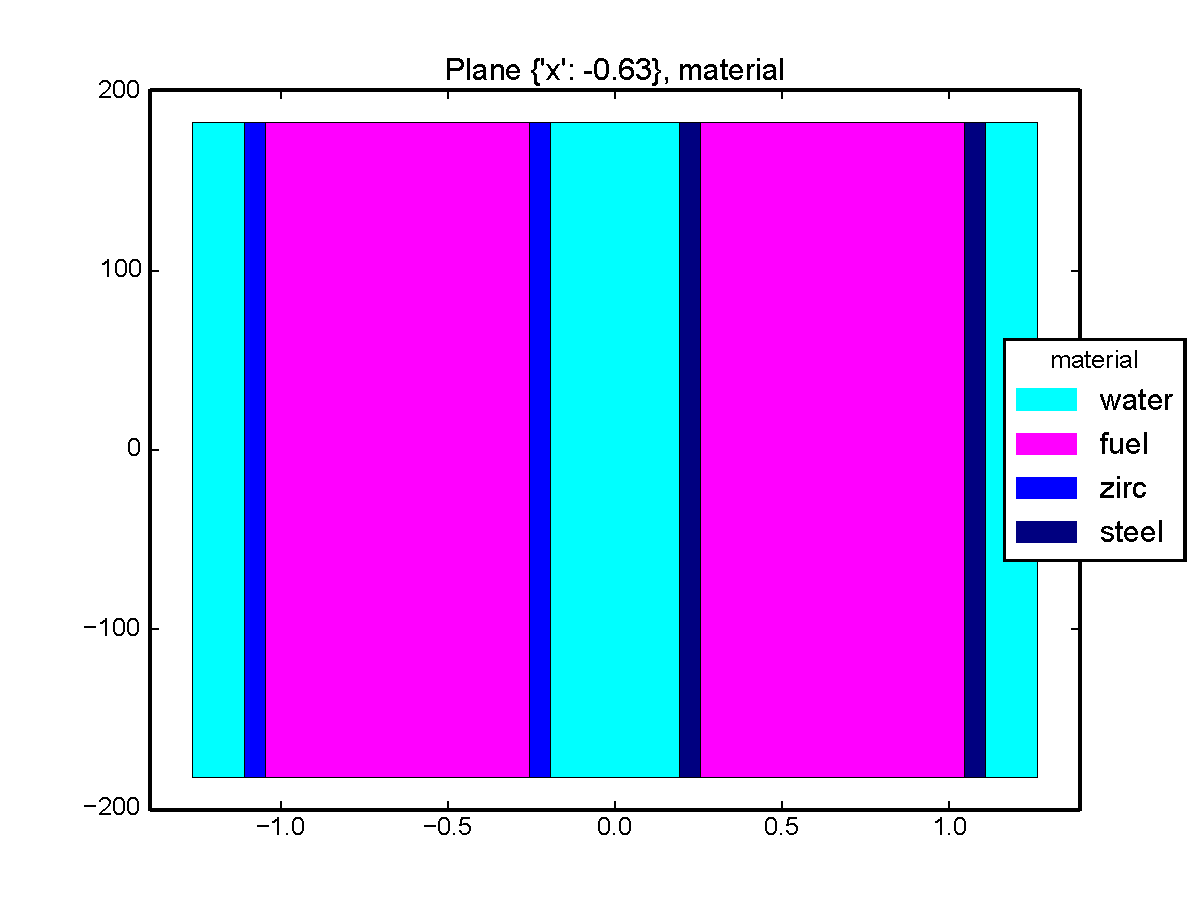
\includegraphics[width=\textwidth]{examples/geom3_px1.pdf}
        \column{0.3\textwidth}
            {\tiny y plane at 1}
            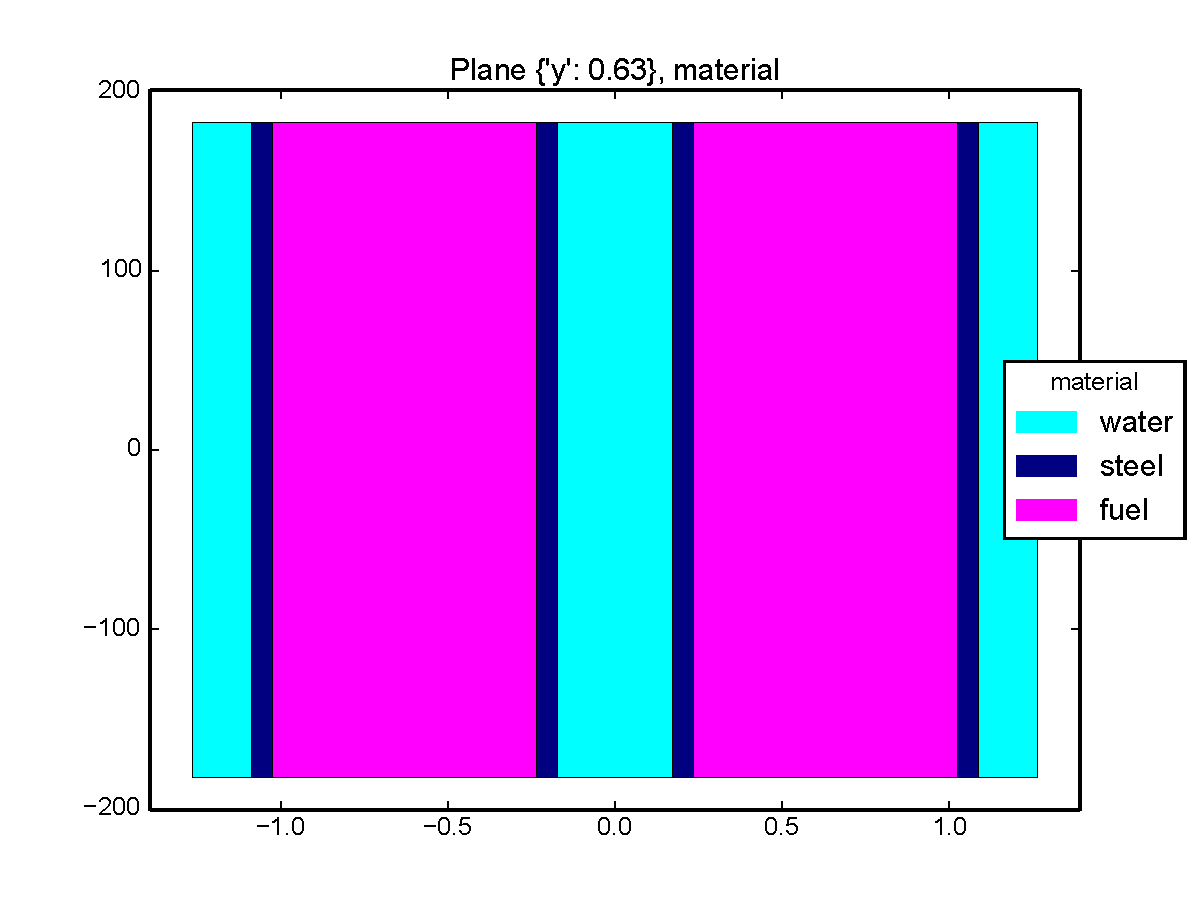
\includegraphics[width=\textwidth]{examples/geom3_py2.pdf}
    \end{columns}
\end{frame}




%%%%%%%%%%%%%%%%%%%%%%%%%%%%%%%%%%%%%%%%%%%%%%%%%%%%%%%%%%%%%%%%%%%%%%%%%%%%%%%%%%%%%%%%%%%%%%%%%%%%%
\subsection{High-level interface to MCNP}
\begin{frame}[fragile]
    \frametitle{High-level interface to MCNP}
    \inputminted[frame=single,fontfamily=tt,fontsize=\footnotesize]{python}{examples/hmcnp1.py}
\end{frame}

\begin{frame}[fragile]
    \frametitle{High-level interface to MCNP: input file}
    \inputminted[frame=single,fontfamily=tt,fontsize=\footnotesize,lastline=18]{rst}{examples/m1_0/i_}
\end{frame}

\begin{frame}[fragile]
    \frametitle{High-level interface to MCNP: input file continued}
    \inputminted[frame=single,fontfamily=tt,fontsize=\footnotesize,firstline=18,lastline=36]{rst}{examples/m1_0/i_}
\end{frame}

\begin{frame}[fragile]
    \frametitle{High-level interface to MCNP: input file continued}
    \inputminted[frame=single,fontfamily=tt,fontsize=\footnotesize,firstline=36]{rst}{examples/m1_0/i_}
\end{frame}

\begin{frame}\frametitle{High-level interface to MCNP: plot 1}
    \includegraphics[width=\textwidth,page=1]{examples/m1_0/i_.pdf}
\end{frame}

%% \begin{frame}\frametitle{High-level interface to MCNP: plot 2}
%%     \includegraphics[width=\textwidth,page=2]{examples/m1_0/i_.pdf}
%% \end{frame}
%% 
%% \begin{frame}\frametitle{High-level interface to MCNP: plot 3}
%%     \includegraphics[width=\textwidth,page=3]{examples/m1_0/i_.pdf}
%% \end{frame}
%% 
\begin{frame}{MCNP-specific data}

    \begin{block}{Data in general model}
        \begin{itemize}
            \item geometry
            \item axial behaviour of system variables (temperature, density -- to define MCNP geometry, heat -- to define tallies)
        \end{itemize}
    \end{block}

    \begin{block}{What else MCNP needs}
        \begin{itemize}
            \item Material specifications
            \item Boundary conditions
            \item Description of (criticality) source
        \end{itemize}
    \end{block}
\end{frame}

\begin{frame}[fragile]
    \frametitle{Material specifications: water}
    \inputminted[frame=single,fontfamily=tt,fontsize=\scriptsize]{python}{examples/mcnp_water.py}
\end{frame}

\begin{frame}[fragile]
    \frametitle{Material specifications: water continued}
    \inputminted[frame=single,fontfamily=tt,fontsize=\scriptsize]{rst}{examples/mcnp_water.log}
\end{frame}

\begin{frame}[fragile]
    \frametitle{Material specifications: steel}
    \inputminted[frame=single,fontfamily=tt,fontsize=\scriptsize]{python}{examples/mcnp_zirc.py}
\end{frame}

\begin{frame}[fragile]
    \frametitle{Material specifications: steel continued}
    \inputminted[frame=single,fontfamily=tt,fontsize=\scriptsize]{rst}{examples/mcnp_zirc.log}
\end{frame}

\begin{frame}[fragile]
    \frametitle{Material specifications: mox}
    \inputminted[frame=single,fontfamily=tt,fontsize=\tiny]{python}{examples/mcnp_mox.py}
\end{frame}

\begin{frame}[fragile]
    \frametitle{Material specifications: mox continued}
    {\tiny before tune() method}
    \inputminted[frame=single,fontfamily=tt,fontsize=\tiny,lastline=13]{rst}{examples/mcnp_mox.log}
    {\tiny after tune() method}
    \inputminted[frame=single,fontfamily=tt,fontsize=\tiny,firstline=14]{rst}{examples/mcnp_mox.log}
\end{frame}

\begin{frame}[fragile]
    \frametitle{Set materials to high-level MCNP interface}
    \inputminted[frame=single,fontfamily=tt,fontsize=\footnotesize]{python}{examples/hmcnp2.py}
\end{frame}

\begin{frame}[fragile]
    \frametitle{MCNP input file}
    \inputminted[frame=single,fontfamily=tt,fontsize=\tiny,lastline=30]{rst}{examples/m2_0/i_}
\end{frame}

\begin{frame}[fragile]
    \frametitle{MCNP input file continued 1}
    \inputminted[frame=single,fontfamily=tt,fontsize=\tiny,firstline=30,lastline=60]{rst}{examples/m2_0/i_}
\end{frame}

\begin{frame}[fragile]
    \frametitle{MCNP input file continued 2}
    \inputminted[frame=single,fontfamily=tt,fontsize=\tiny,firstline=60,lastline=90]{rst}{examples/m2_0/i_}
\end{frame}

\begin{frame}[fragile]
    \frametitle{MCNP input file continued 3}
    \inputminted[frame=single,fontfamily=tt,fontsize=\tiny,firstline=106]{rst}{examples/m2_0/i_}
\end{frame}

\begin{frame}\frametitle{MCNP plot 1}
    \includegraphics[width=\textwidth,page=1]{examples/m2_0/i_.pdf}
\end{frame}

\begin{frame}\frametitle{MCNP plot 2}
    \includegraphics[width=\textwidth,page=2]{examples/m2_0/i_.pdf}
\end{frame}

\begin{frame}\frametitle{MCNP plot 3}
    \includegraphics[width=\textwidth,page=3]{examples/m2_0/i_.pdf}
\end{frame}

\begin{frame}[fragile]
    \frametitle{Set boundary conditions to high-level MCNP interface}
    \inputminted[frame=single,fontfamily=tt,fontsize=\footnotesize]{python}{examples/hmcnp3.py}
\end{frame}

\begin{frame}[fragile]
    \frametitle{MCNP input file}
    \begin{columns}
        \column{0.5\textwidth}
        {\tiny without boundary conditions}
        \inputminted[frame=single,fontfamily=tt,fontsize=\tiny,firstline=28,lastline=43]{rst}{examples/m2_0/i_}
        \column{0.5\textwidth}
        {\tiny with boundary conditions}
        \inputminted[frame=single,fontfamily=tt,fontsize=\tiny,firstline=28,lastline=48]{rst}{examples/m3_0/i_}
    \end{columns}
\end{frame}

\begin{frame}[fragile]
    \frametitle{Specify additional cards for MCNP input}
    \inputminted[frame=single,fontfamily=tt,fontsize=\tiny]{python}{examples/hmcnp4.py}
\end{frame}

\begin{frame}[fragile]
    \frametitle{MCNP input file}
    {\tiny Additional cell cards}
    \inputminted[frame=single,fontfamily=tt,fontsize=\tiny,firstline=29,lastline=32]{rst}{examples/m4_0/i_}

    {\tiny Additional surface cards}
    \inputminted[frame=single,fontfamily=tt,fontsize=\tiny,firstline=49,lastline=55]{rst}{examples/m4_0/i_}

    {\tiny Additional data cards}
    \inputminted[frame=single,fontfamily=tt,fontsize=\tiny,firstline=129]{rst}{examples/m4_0/i_}
\end{frame}

\begin{frame}[fragile]
    \frametitle{Tallies for MCNP input}
    \inputminted[frame=single,fontfamily=tt,fontsize=\tiny]{python}{examples/hmcnp5.py}
\end{frame}

\begin{frame}[fragile]
    \frametitle{MCNP input file with tallies}
    \inputminted[frame=single,fontfamily=tt,fontsize=\tiny,firstline=130]{rst}{examples/m5_0/i_}
\end{frame}

\begin{frame}[fragile]
    \frametitle{MCNP meshtal file}
    \inputminted[frame=single,fontfamily=tt,fontsize=\tiny,firstline=30,lastline=60]{rst}{examples/m5_0/meshtal}
\end{frame}

\begin{frame}[fragile]
    \frametitle{MCNP results}
    \begin{columns}
        \column{0.5\textwidth}
        {\tiny x plane at -1}
        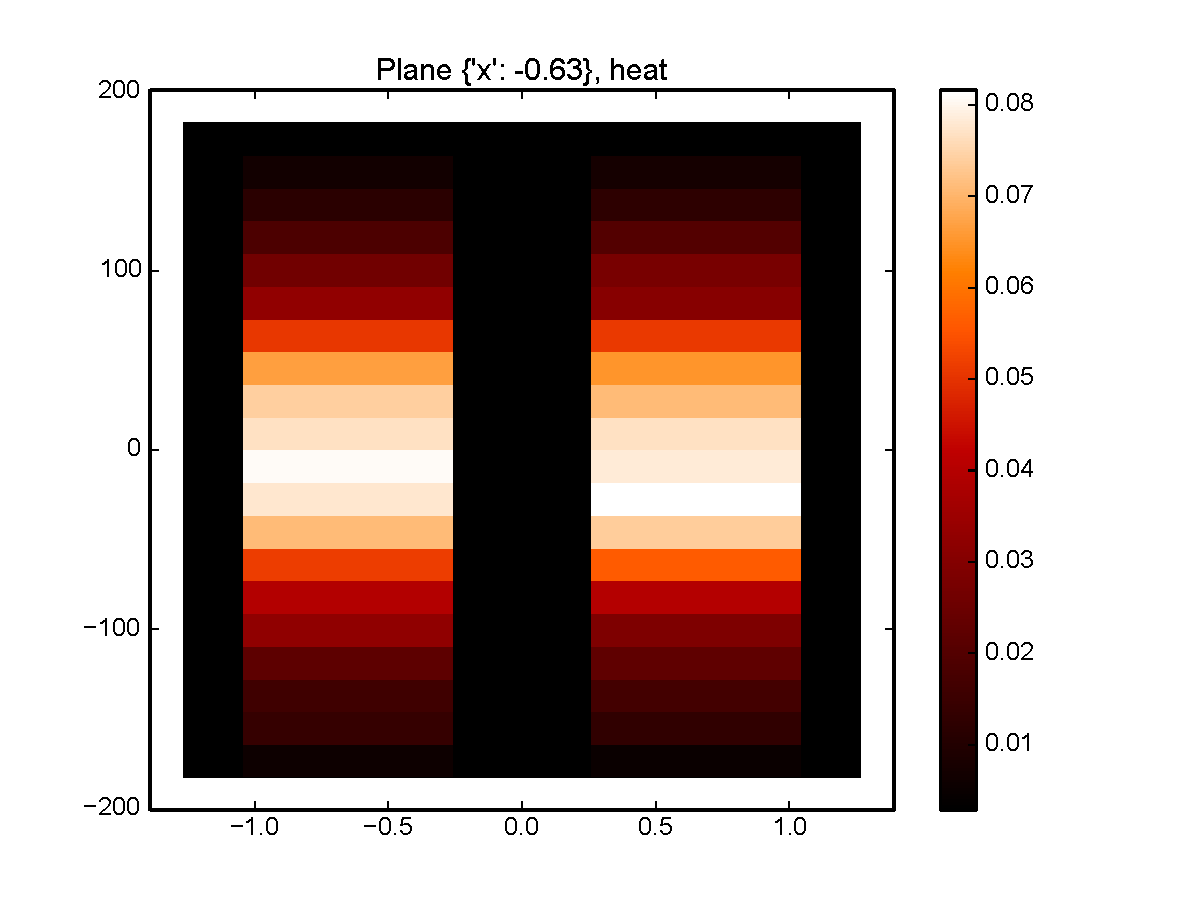
\includegraphics[width=\textwidth]{examples/hmcnp5_hx1.pdf}
        \column{0.5\textwidth}
        {\tiny x plane at 1}
        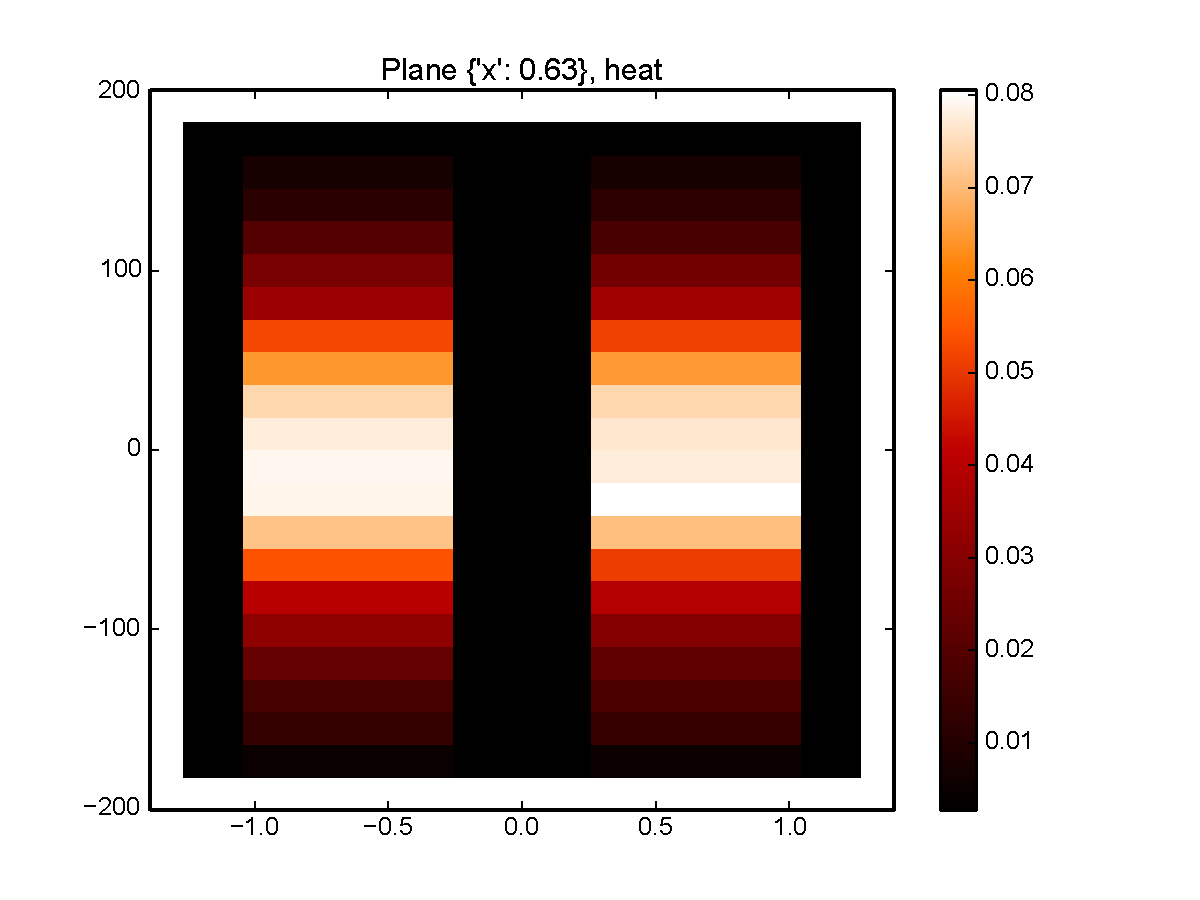
\includegraphics[width=\textwidth]{examples/hmcnp5_hx2.pdf}
    \end{columns}
\end{frame}




%%%%%%%%%%%%%%%%%%%%%%%%%%%%%%%%%%%%%%%%%%%%%%%%%%%%%%%%%%%%%%%%%%%%%%%%%%%%%%%%%%%%%%%%%%%%%%%%%%%%%
\subsection{High-level interface to SCF}
\begin{frame}[fragile]
    \frametitle{High-level interface to SCF}
    \inputminted[frame=single,fontfamily=tt,fontsize=\footnotesize]{python}{examples/hscf1.py}

    \begin{block}{Limitations}
        \begin{itemize}
            \item Rectangular container (i.e. an instance of the pirs.solids.Box() class)
            \item Rods inserted into grid element centers, no empty grid elements.
            \item Container and rods (and all internal structure) have the same height.
        \end{itemize}
    \end{block}
\end{frame}

\begin{frame}[fragile]
    \frametitle{SCF input file: channels}
    \inputminted[frame=single,fontfamily=tt,fontsize=\tiny,firstline=92,lastline=117]{rst}{examples/s1_0/input.txt}
\end{frame}

\begin{frame}[fragile]
    \frametitle{SCF input file: rods}
    \inputminted[frame=single,fontfamily=tt,fontsize=\tiny,firstline=152,lastline=166]{rst}{examples/s1_0/input.txt}
\end{frame}

\begin{frame}[fragile]
    \frametitle{SCF input file: power axial profile}
    \inputminted[frame=single,fontfamily=tt,fontsize=\tiny,firstline=343,lastline=362]{rst}{examples/s1_0/input.txt}
\end{frame}

\begin{frame}[fragile]
    \frametitle{SCF-specific parameters}
    \inputminted[frame=single,fontfamily=tt,fontsize=\tiny]{python}{examples/hscf2.py}
\end{frame}


\begin{frame}[fragile]
    \frametitle{SCF-specific parameters: rod material specifications}
    \inputminted[frame=single,fontfamily=tt,fontsize=\tiny]{python}{examples/hscf3.py}
\end{frame}

\begin{frame}[fragile]
    \frametitle{SCF-specific parameters: SCF results}
    \begin{columns}
        \column{0.5\textwidth}
        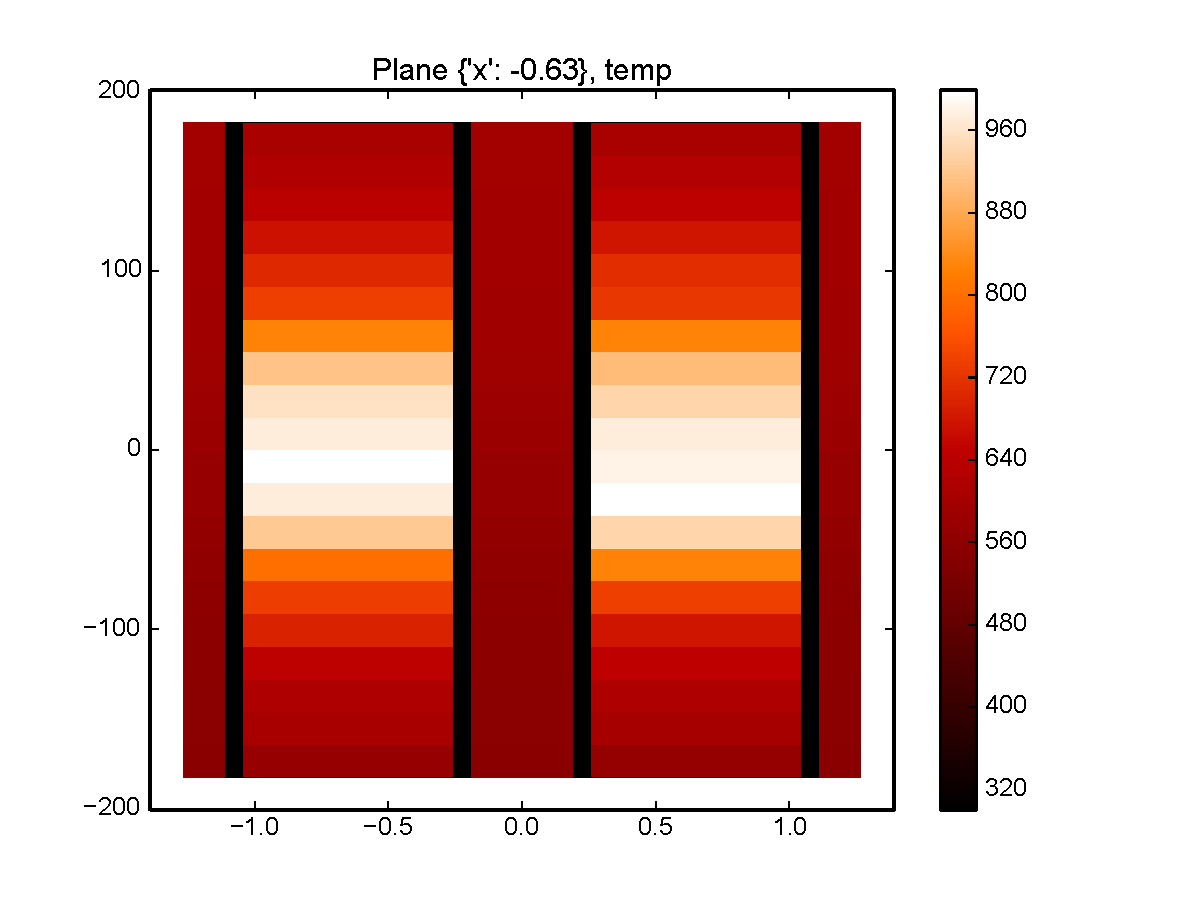
\includegraphics[width=\textwidth]{examples/hscf3_tx1.pdf}
        \column{0.5\textwidth}
        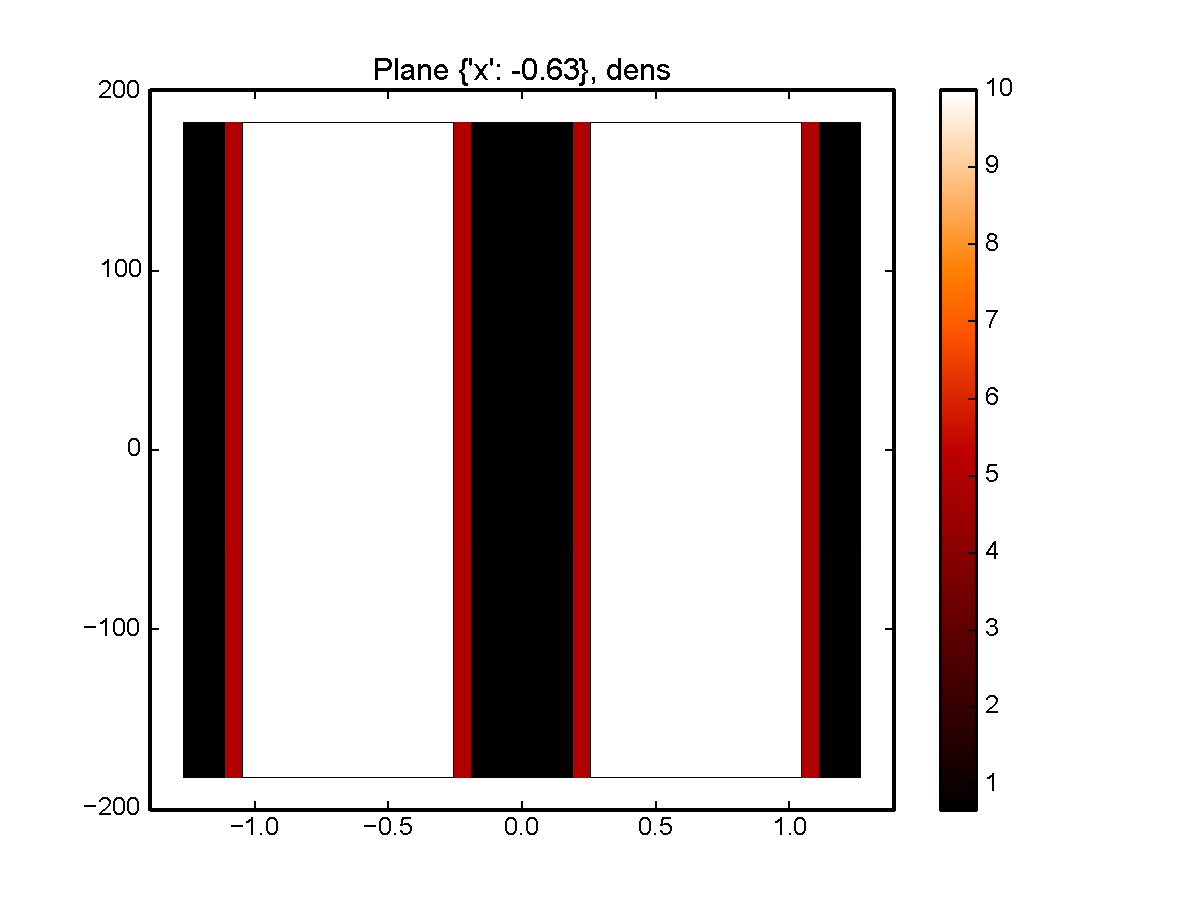
\includegraphics[width=\textwidth]{examples/hscf3_dx1.pdf}
    \end{columns}
\end{frame}


\begin{frame}[fragile]
    \frametitle{Data exchange between interfaces}
    \inputminted[frame=single,fontfamily=tt,fontsize=\tiny,lastline=27]{python}{examples/coupling.py}
\end{frame}



%%%%%%%%%%%%%%%%%%%%%%%%%%%%%%%%%%%%%%%%%%%%%%%%%%%%%%%%%%%%%%%%%%%%%%%%%%%%%%%%%%%%%%%%%%%%%%%%%%%%%
% \section{Results for PWR assembly}
%\begin{frame}{PWR assembly model}
    \includegraphics[width=\textwidth]{examples/res_model.pdf}
\end{frame}

\begin{frame}{PWR assembly model}
    \begin{itemize}
        \item Computed on IC2 cluster
        \item Initial statistics 5000 10 100
        \item Conv. criteria: Keff, Tfuel.
        \item Statistics at 56-th iteration: 149227 10 100
        \item MCNP input: 12K cells, 18K lines.
    \end{itemize}
\end{frame}

\begin{frame}{Keff vs. iterations}
    \includegraphics[width=\textwidth]{examples/res_keff.pdf}
\end{frame}

\begin{frame}{dTf vs. iterations}
    Maximal change in fuel temperature from I-1-th to I-th iteration
    \includegraphics[width=\textwidth]{examples/res_dTf.pdf}
\end{frame}

\begin{frame}{Relaxation factor vs. iterations}
    \includegraphics[width=\textwidth]{examples/res_alpha.pdf}
\end{frame}


\begin{frame}{Power profile}
    \includegraphics[width=\textwidth]{examples/res_hx.pdf}
\end{frame}

\begin{frame}{Power profile}
    \includegraphics[width=\textwidth]{examples/res_hz.pdf}
\end{frame}

\begin{frame}{Fuel temperature profile}
    \includegraphics[width=\textwidth]{examples/res_tx.pdf}
\end{frame}



%%%%%%%%%%%%%%%%%%%%%%%%%%%%%%%%%%%%%%%%%%%%%%%%%%%%%%%%%%%%%%%%%%%%%%%%%%%%%%%%%%%%%%%%%%%%%%%%%%%%%
\section{Results for 3x3 minicore}
\begin{frame}{3x3 minicore model}
    \includegraphics[width=\textwidth]{examples/a_model_z.pdf}
\end{frame}

\begin{frame}{PWR assembly model}
    \begin{itemize}
        \item PIRS deployed on a cluster, MCNP jobs queued to a job submission system
        \item Long MCNP initialization time due to huge amount of cells 
        \item Good agreement with other results (see D1.9)
    \end{itemize}
\end{frame}


\begin{frame}{Results, vertical profile}
    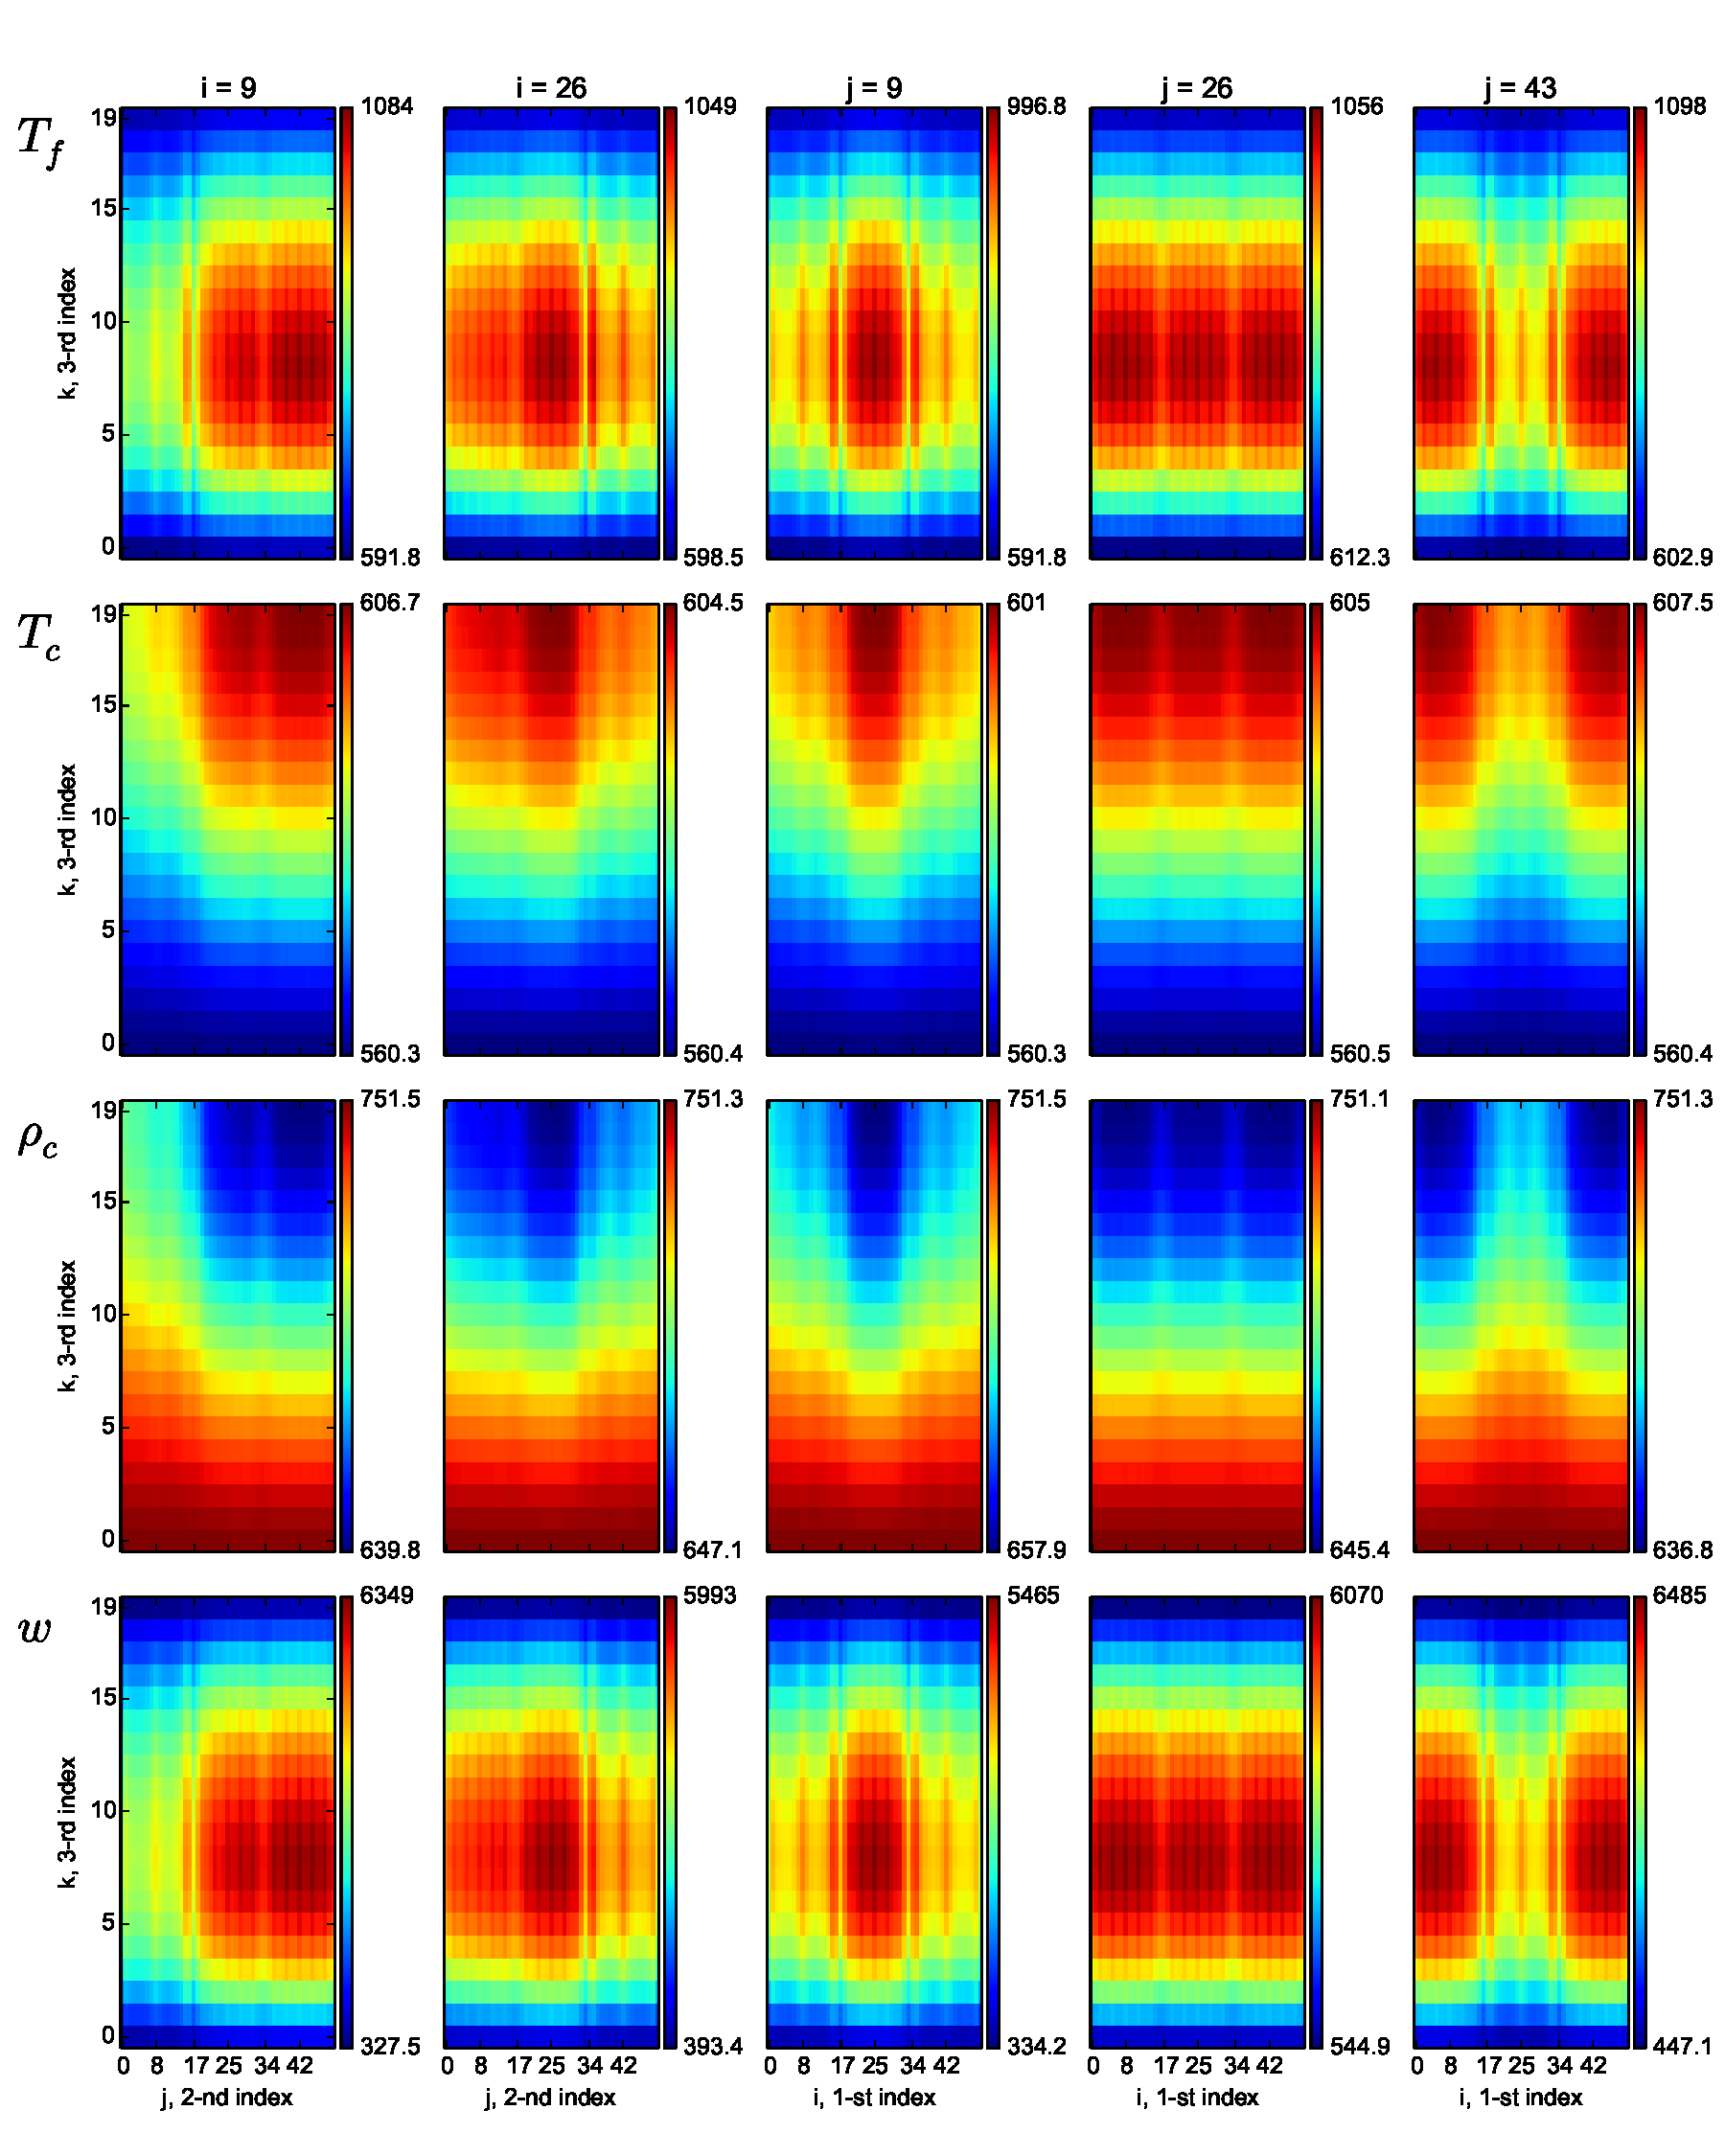
\includegraphics[width=0.5\textwidth]{examples/map_anton_i.pdf}
\end{frame}

\begin{frame}{Results, horizontal profile}
    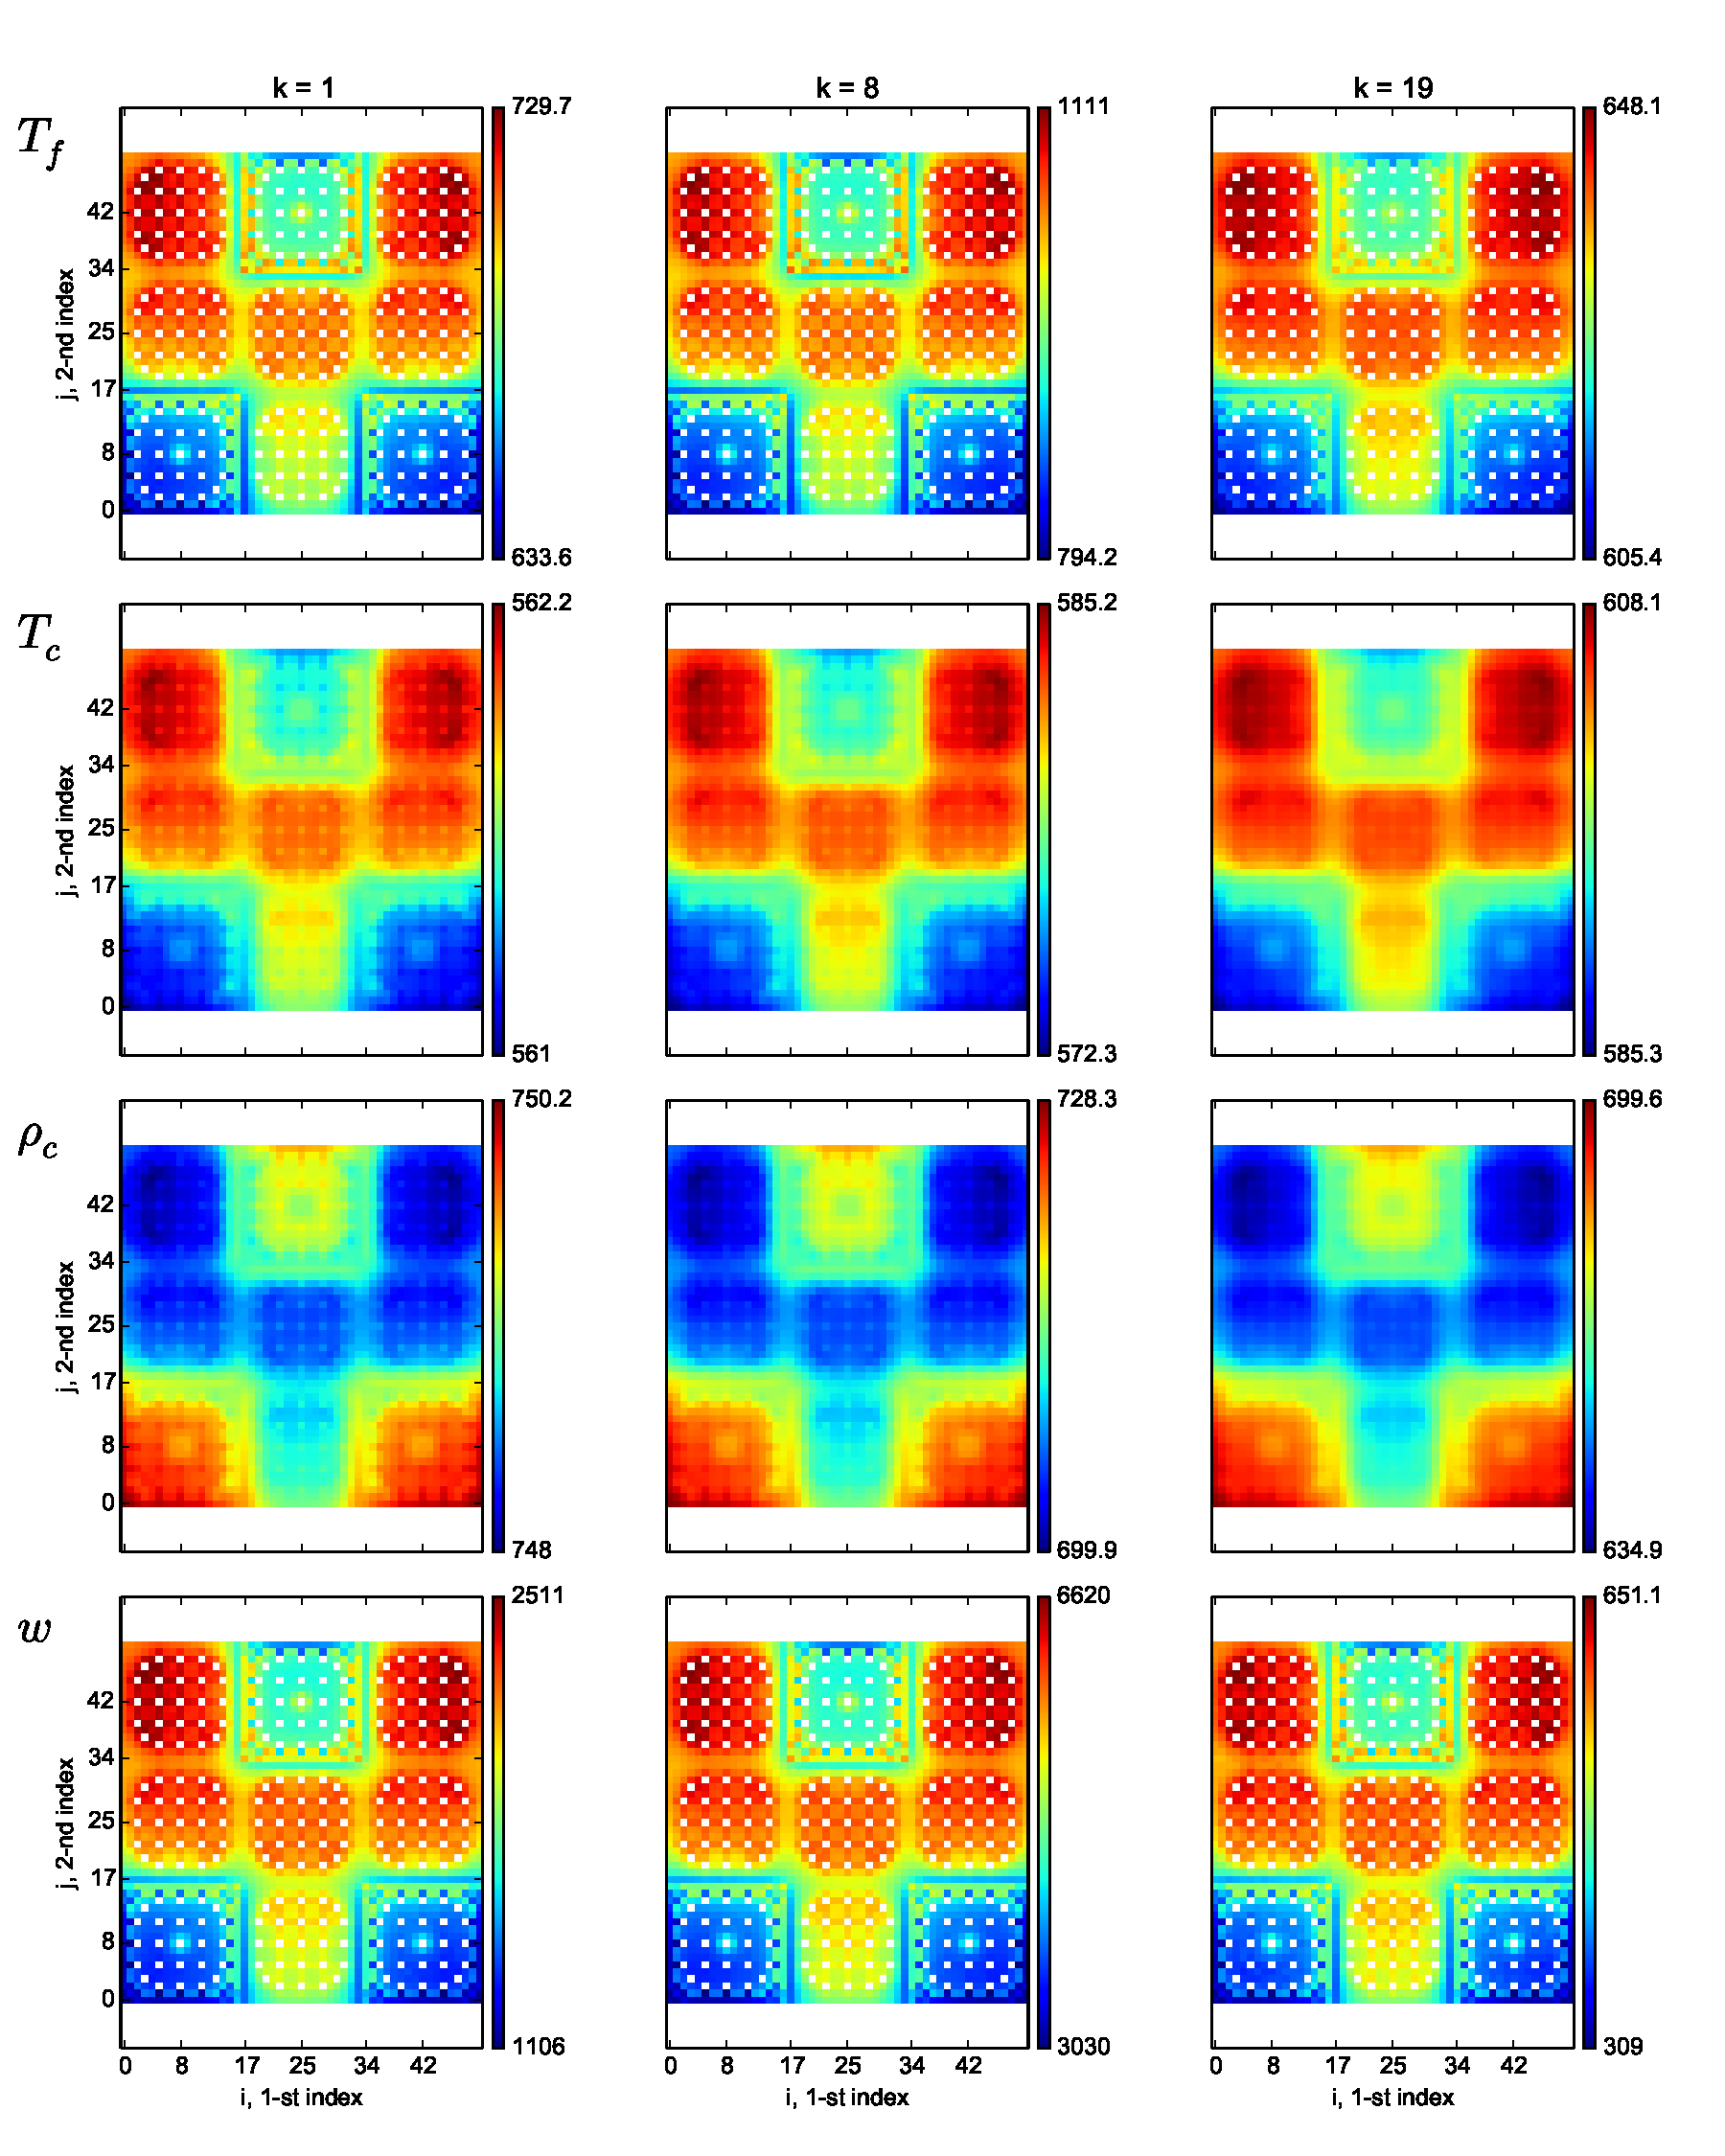
\includegraphics[width=0.5\textwidth]{examples/map_anton_k.pdf}
\end{frame}



%%%%%%%%%%%%%%%%%%%%%%%%%%%%%%%%%%%%%%%%%%%%%%%%%%%%%%%%%%%%%%%%%%%%%%%%%%%%%%%%%%%%%%%%%%%%%%%%%%%%%
\section{Conclusions and outlook}
\include{seminar_conc}

\end{document}
